\documentclass[10pt,a4paper]{article}
\usepackage[bindingoffset=0.2in,%
            left=2.5cm,right=2cm,top=2.7cm,bottom=1in,%
            footskip=.25in]{geometry}
\usepackage[utf8]{inputenc}
\usepackage[ngerman]{babel}
\usepackage{amsmath, amsfonts, amssymb}
\usepackage{scrpage2}
\usepackage{color}
\usepackage{titlesec}
\pagestyle{scrheadings}
\usepackage{ulem, contour}
\usepackage{multicol}
\usepackage{hyperref}
\usepackage{listings}
\usepackage{pdfpages}
\usepackage{tabularx}
\usepackage{subcaption}
\usepackage{float}
\usepackage{scrextend}
\usepackage{enumerate}
\usepackage{footmisc}
\usepackage{multirow}
\usepackage{csquotes}

\usepackage[style=authoryear, backend=biber]{biblatex}
\addbibresource{bibliography.bib}

\DeclareFixedFont{\ttb}{T1}{txtt}{bx}{n}{12} % for bold
\DeclareFixedFont{\ttm}{T1}{txtt}{m}{n}{12}  % for normal

\renewcommand{\ULdepth}{1.8pt}
\contourlength{0.8pt}

\newcommand{\cul}[1]{%
  \uline{\phantom{#1}}%
  \llap{\contour{white}{#1}}%
}

\graphicspath{
    {Images/}
    {gnuplot/Spannung/}
}

\newrobustcmd*{\parentexttrack}[1]{%
  \begingroup
  \blx@blxinit
  \blx@setsfcodes
  \blx@bibopenparen#1\blx@bibcloseparen
  \endgroup}

\AtEveryCite{%
  \let\parentext=\parentexttrack%
  \let\bibopenparen=\bibopenbracket%
  \let\bibcloseparen=\bibclosebracket}

\definecolor{gray}{rgb}{0.33, 0.33, 0.33}
\definecolor{greengreen}{rgb}{0.0, 0.56, 0.0}
\definecolor{fgreen}{rgb}{0.13, 0.55, 0.13}
\definecolor{grellow}{rgb}{0.68, 1.0, 0.18}
\definecolor{orange}{rgb}{1.0, 0.49, 0.0}
\definecolor{deepblue}{rgb}{0,0,0.5}
\definecolor{deepred}{rgb}{0.6,0,0}
\definecolor{deepgreen}{rgb}{0,0.5,0}

\usepackage{pifont}

\newcommand{\cmark}{\ding{51}}%
\newcommand{\xmark}{\ding{55}}%
\newcommand{\wontfix}{\rlap{$\square$}{\large\hspace{1pt}\xmark}}


\newcommand{\vnr}{8}
\newcommand{\anr}{1}

\ihead{}
\ohead{Anfängerpraktikum 2}
\chead{Versuch \vnr, Abgabe \anr : Auf- \& Entladung Kondensator}
\cfoot{\pagemark}
\setheadsepline{.5pt}
\setlength\parindent{0pt}

\begin{document}

\begin{multicols}{2}
\begin{labeling}{Versuch-Nr.:}
\item[\textcolor{white}{x}Protokollant:\hspace{38pt}] \cul{Name} \wontfix
\item[\textcolor{white}{x}Zusammenarbeit\footnotemark mit:] \cul{Name} $\square$
\item[\textcolor{white}{x}Datum:\hspace{62pt}] \cul{\today}

\columnbreak

\item[Kurs: \hspace{27pt}] \cul{Anfängerpraktikum 2}
\item[Assistent: \hspace{8.7pt}] \cul{Name}
\item[Versuch-Nr.:] \underline{\vnr}
\end{labeling}
\end{multicols}

\begin{figure}[h]
\hspace{-0.5cm}\centerline{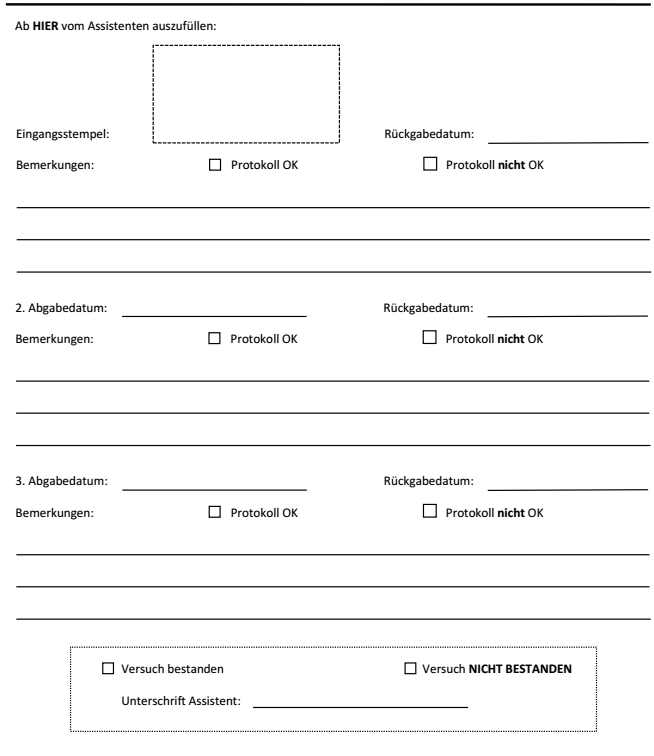
\includegraphics[width=1.1\linewidth , height=19cm]{Deckblatt_rest}}
\end{figure}

\newpage

\tableofcontents

\vspace{10pt}

\section{Schaltbild}
\begin{flushleft}
\begin{figure}[h]
\centering
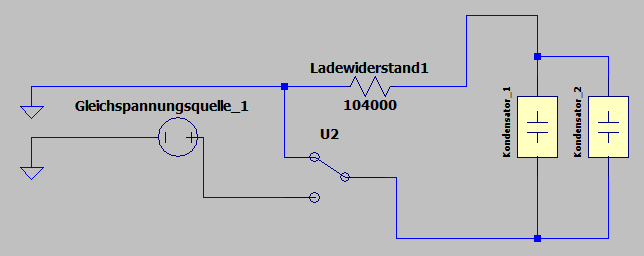
\includegraphics[scale=0.5]{Schaltbild_prallel}
\caption{Schaltbild der Simulationssoftware}
\label{fig:Schaltbild}
\end{figure}
Das Schaltbild (Abbildung \ref{fig:Schaltbild}) zeigt das Simulationsschaltbild für die Parallelschaltung der Kondensatoren. Die anderen Schaltungen sind analog zu diesem aufgebaut.
\end{flushleft}

\section{Bestimmung der Kapazitäten}
\begin{flushleft}
Wir bestimmen die Kapazität mittels des Stromes \textit{I}, der an dem jeweiligen Kondensator(en) anliegt. Dabei gehen wir so vor, dass wir zunäcsht den maximalen Stromfluss ablesen und dann den Zeitpunkt bestimmen, wann dieser Strom auf seinen $e$-ten Teil abgefallen ist. Für diese Zeitdifferenz $t$ zwischen den beiden Messpunkten gilt:
\begin{equation}\label{eq:capa}
t = R \cdot C \Rightarrow C = \frac{t}{R}
\end{equation}

Dabei nehmen wir wie bereits erwähnt $I_1(t) = max(I(t))$, da dieser Punkt sehr einfach abzulesen ist (geringer Fehler!). Anschließend berechnen wir den $e$-ten Teil udn bestimmen die Zeitdifferenz mit:
\begin{equation}\label{eq:epart}
\frac{I_2(t)}{I_1(t)} = \frac{1}{e} \Rightarrow I_2(t) = \frac{I_1(t)}{e}
\end{equation}
\end{flushleft}

\subsection{Messergebnisse}
\begin{flushleft}

Wir führen die Messungen zur Bestimmung der Kapazität beim Aufalden des Kondensators durch. Die Berechnungen beim Entladen sind (fast - Formeln nicht) identisch und führen zu den gleichen Ergebnissen und somit redundant.

\newpage

\begin{table}[h]
\centering
\caption{Messergebnisse}
\label{tab:messerg}
\begin{tabular}{|c|c|c|c|c|c|}
\hline
Kapazität & $I_1(t) [\mu A]$ & $I_2(t) [\mu A]$ & $ t_1 [s]$ & $t_2 [s]$ & $t_{diff} [s]$ \\
\hline
$C_1$ & 95.648 & $\approx$ 35.187 & 0.6 & 11 & 10.4  \\
\hline
$C_1$ & 95.659 & $\approx$ 35.191 & 0.6 & 11.25 & 10.65 \\
\hline
$C_1 \parallel C_2$ & 48.5195 & $\approx$ 17.849 & 0.6 & 21.657 & 21.057 \\
\hline
$C_1 - C_2$ & 96.138 & $\approx$ 35.367 & 0.551 & 5.8146 & 5.2636 \\
\hline
\end{tabular}
\end{table}

Anhand der Messwerte aus Tabelle \ref{tab:messerg} ist bereits zu erkennen, dass $C_1$ und $C_2$ gleiche Kapazitäten besitzen. Weiterhin ist zu sehen, dass die Zeitdifferenz des Abfalls des Stromes bei der Parallelschaltung in etwa das Doppelte der Zeitdifferenz für $C_1$ bzw. $C_2$ und bei der Reihenschaltung etwa die Hälfte beträgt.
\end{flushleft}

\subsection{Berechnungen}
\begin{flushleft}
Mit den ermittelten Messergebnissen (Tabelle \ref{tab:messerg}) könenn wir nun die Kapazitäten mit Formel \ref{eq:capa} bestimmen. In unserem Simulationsversuch beträgt der Widerstand dabei $R = 104k\Omega = 104000 \Omega$ (fest).

\begin{align*}
C_1 &= \frac{t_{diff, C_1}}{R} = \frac{10.4 s}{104000 \Omega} = 1 \cdot 10^{-4} F = 100 \mu F \\
C_2 &= \frac{t_{diff, C_2}}{R} = \frac{10.65 s}{104000 \Omega} \approx 1.024 \cdot 10^{-4} F \approx 102 \mu F \\
C_{para} &= \frac{t_{diff, C_{para}}}{R} = \frac{21.057 s}{104000 \Omega} \approx 2.025 \cdot 10^{-4} F = 203 \mu F \\
C_{reihe} &= \frac{t_{diff, C_{reihe}}}{R} = \frac{5.2636 s}{104000 \Omega} \approx 5,061 \cdot 10^{-5} F = 51 \mu F \\
\end{align*}

Wir erkennen, dass die Kapazität der Kondensatoren $C_1$ und $C_2$ nahezu identisch ist. Wir können annehmen, dass es sich um kapazitätsgleiche Kondensatoren handelt (Im folgenden werden $C_1$ und $C_2$ als $C_1$ bezeichnet).

Weiterhin ist zu erkennen, dass die Kapazität der reihenschaltung doppelt so groß ist wie die von $C_1$ und die Kapazität der Reihenschaltung halb so groß.
\end{flushleft}

\section{Graphen}
\begin{flushleft}
Die im Folgenden gezeigten Graphen sind mit dem Simulationsprogramm \textbf{LTSpice} entstanden.
\end{flushleft}

\subsection{Kondensator $C_1$}
\begin{flushleft}
\begin{figure}[H]
\centering
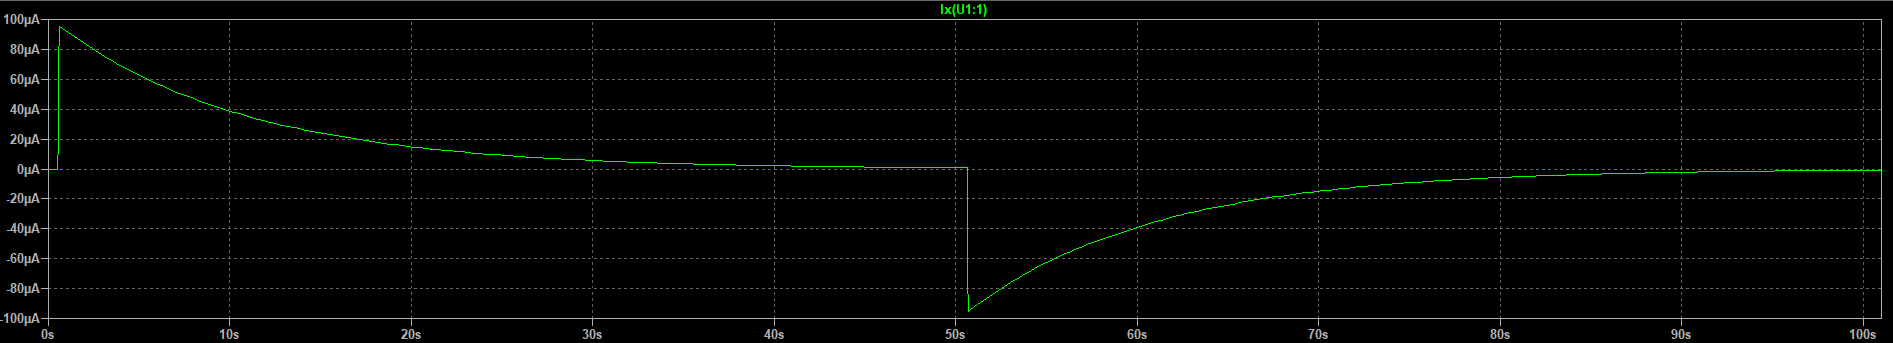
\includegraphics[scale=0.3]{I_C_1}
\caption{Strom beim Auf- und Entladen des Kondensatoren $C_1$.}
\end{figure}

\newpage

\begin{figure}[H]
\centering
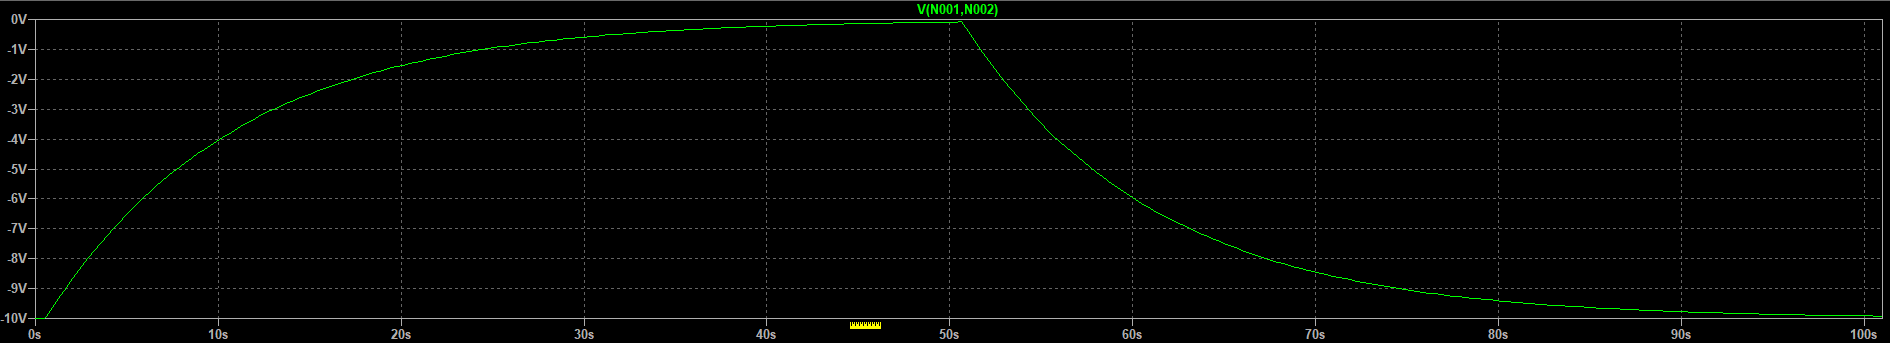
\includegraphics[scale=0.3]{V_C_1}
\caption{Spannung des Kondensators $C_1$ beim Auf- und Entladen.}
\end{figure}
\end{flushleft}

\subsection{Kondensator $C_2$}
\begin{flushleft}
\begin{figure}[H]
\centering
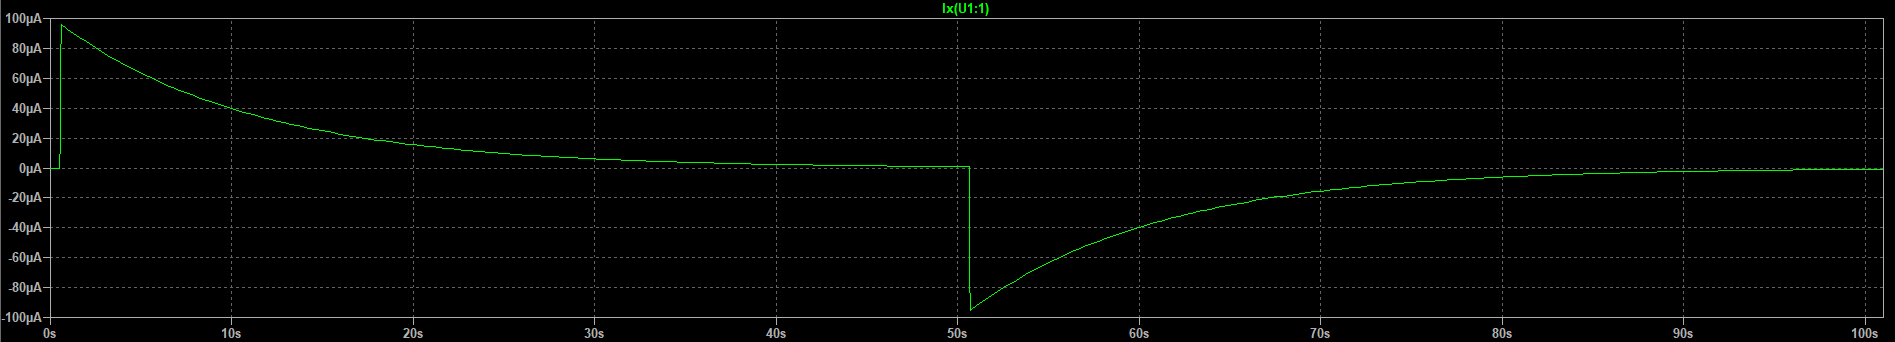
\includegraphics[scale=0.3]{I_C_2}
\caption{Strom beim Auf- und Entladen des Kondensatoren $C_2$.}
\end{figure}

\begin{figure}[H]
\centering
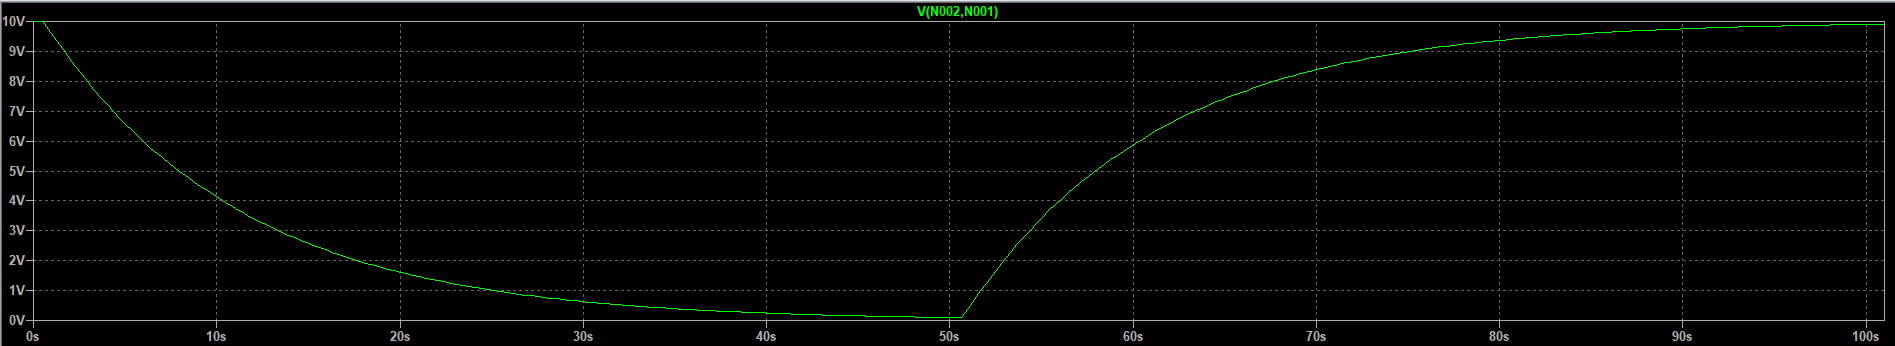
\includegraphics[scale=0.3]{V_C_2}
\caption{Spannung des Kondensators $C_2$ beim Auf- und Entladen.}
\end{figure}
\end{flushleft}

\subsection{Parallelschaltung}
\begin{flushleft}
\begin{figure}[H]
\centering
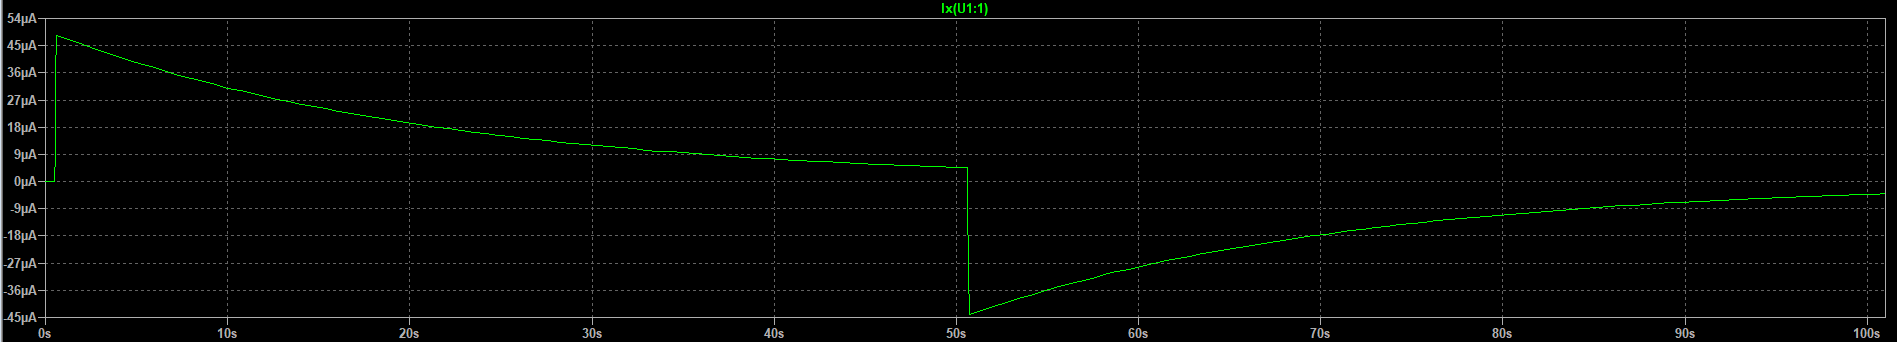
\includegraphics[scale=0.3]{I_C_para}
\caption{Strom beim Auf- und Entladen des Kondensatoren $C_{para}$.}
\end{figure}

\begin{figure}[H]
\centering
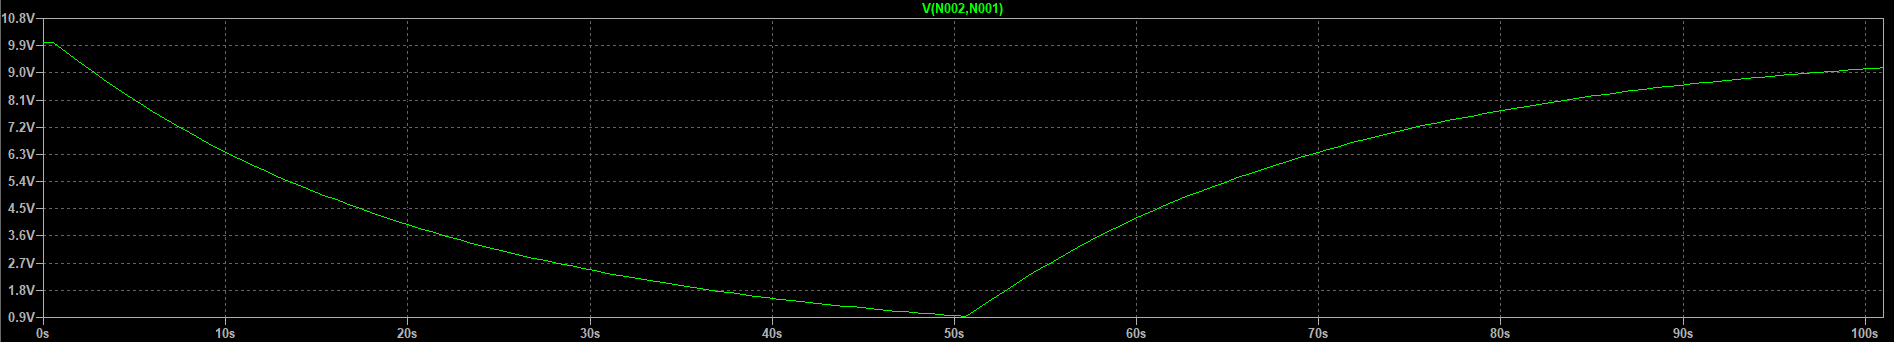
\includegraphics[scale=0.3]{V_C_para}
\caption{Spannung des Kondensators $C_{para}$ beim Auf- und Entladen.}
\end{figure}
\end{flushleft}

\subsection{Reihenschaltung}
\begin{flushleft}
\begin{figure}[H]
\centering
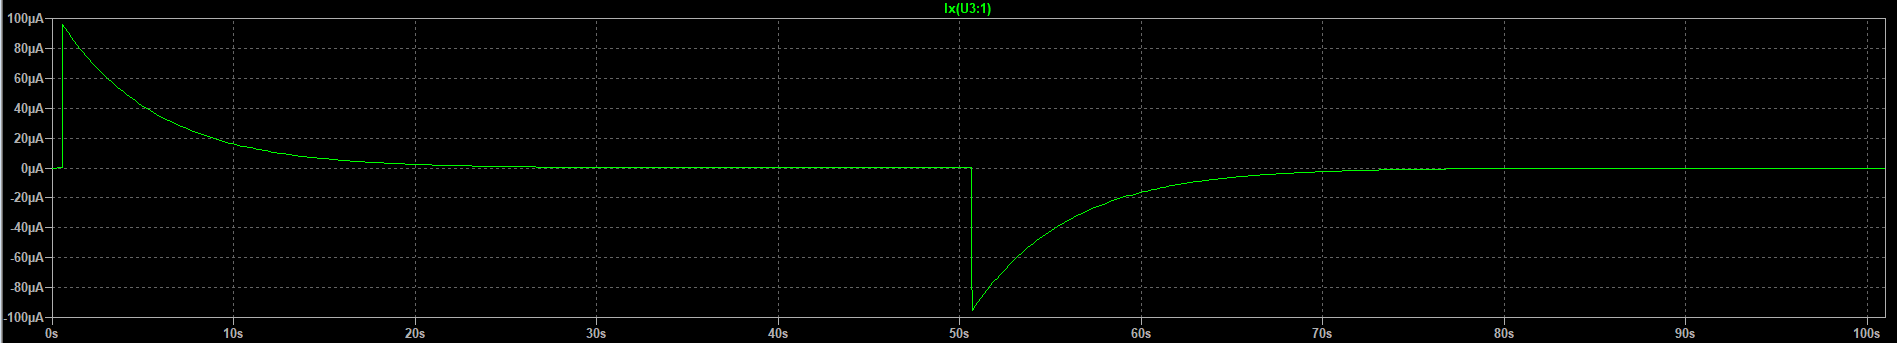
\includegraphics[scale=0.3]{I_C_reihe}
\caption{Strom beim Auf- und Entladen des Kondensatoren $C_{reihe}$.}
\end{figure}

\begin{figure}[H]
\centering
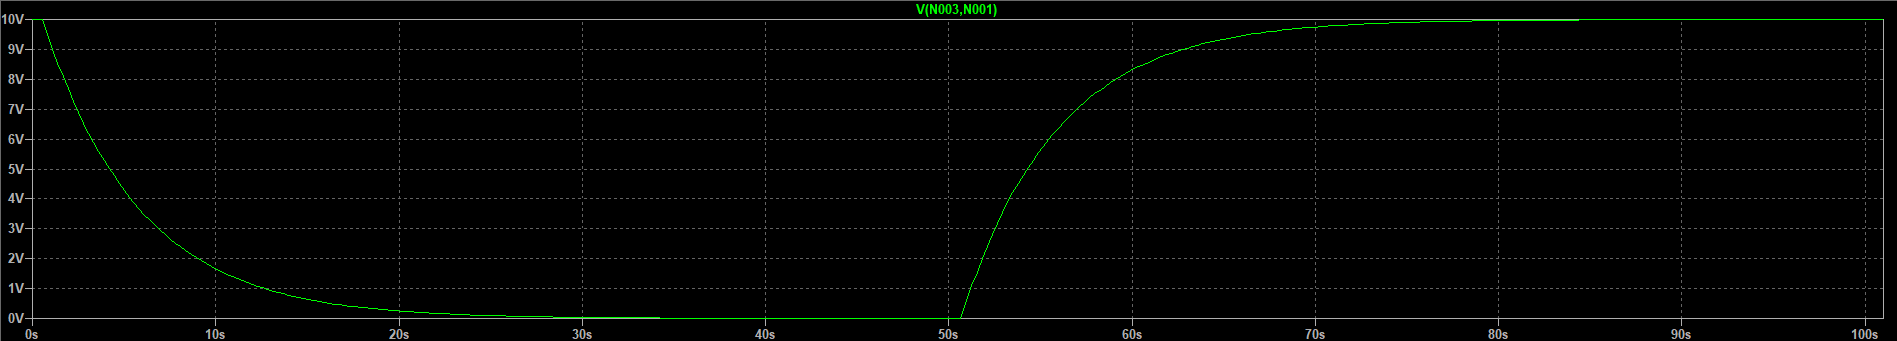
\includegraphics[scale=0.3]{V_C_reihe}
\caption{Spannung des Kondensators $C_{reihe}$ beim Auf- und Entladen.}
\end{figure}
\end{flushleft}

\section{Halblogarithmische Auswertung}
\begin{flushleft}
Die lineare Regression der halblogarithmischen Darstellung der oben gezeigten Graphen bietet eine weitere Möglichkeit die Kapazitäten der Kondensatoren zu bestimmen. Wir betrachten dieses Verfahren für die Kondensatoren $C_1$ und $C_2$, wobei wir die Daten von Kondensator $C_2$ verwendet haben. Beide Kurven unterscheiden sich jedoch nur minimal (die Kapazitäten sind aber gleich).

Weiterhin sind die Darstellungen in zwei Graphen aufgeteilt für Strom und Spannung. Dabei sind jeweils die ersten 50 Sekunden der Daten genutzt, da bei der Simulation nach 50 Sekunden das Auf- und Entladen umegschalten wurde, wodurch sich die Kurvenverläufe ändern und \textbf{nicht} zusammen einer linearen Regression unterzogen werden können! 

\begin{figure}[H]
\centering
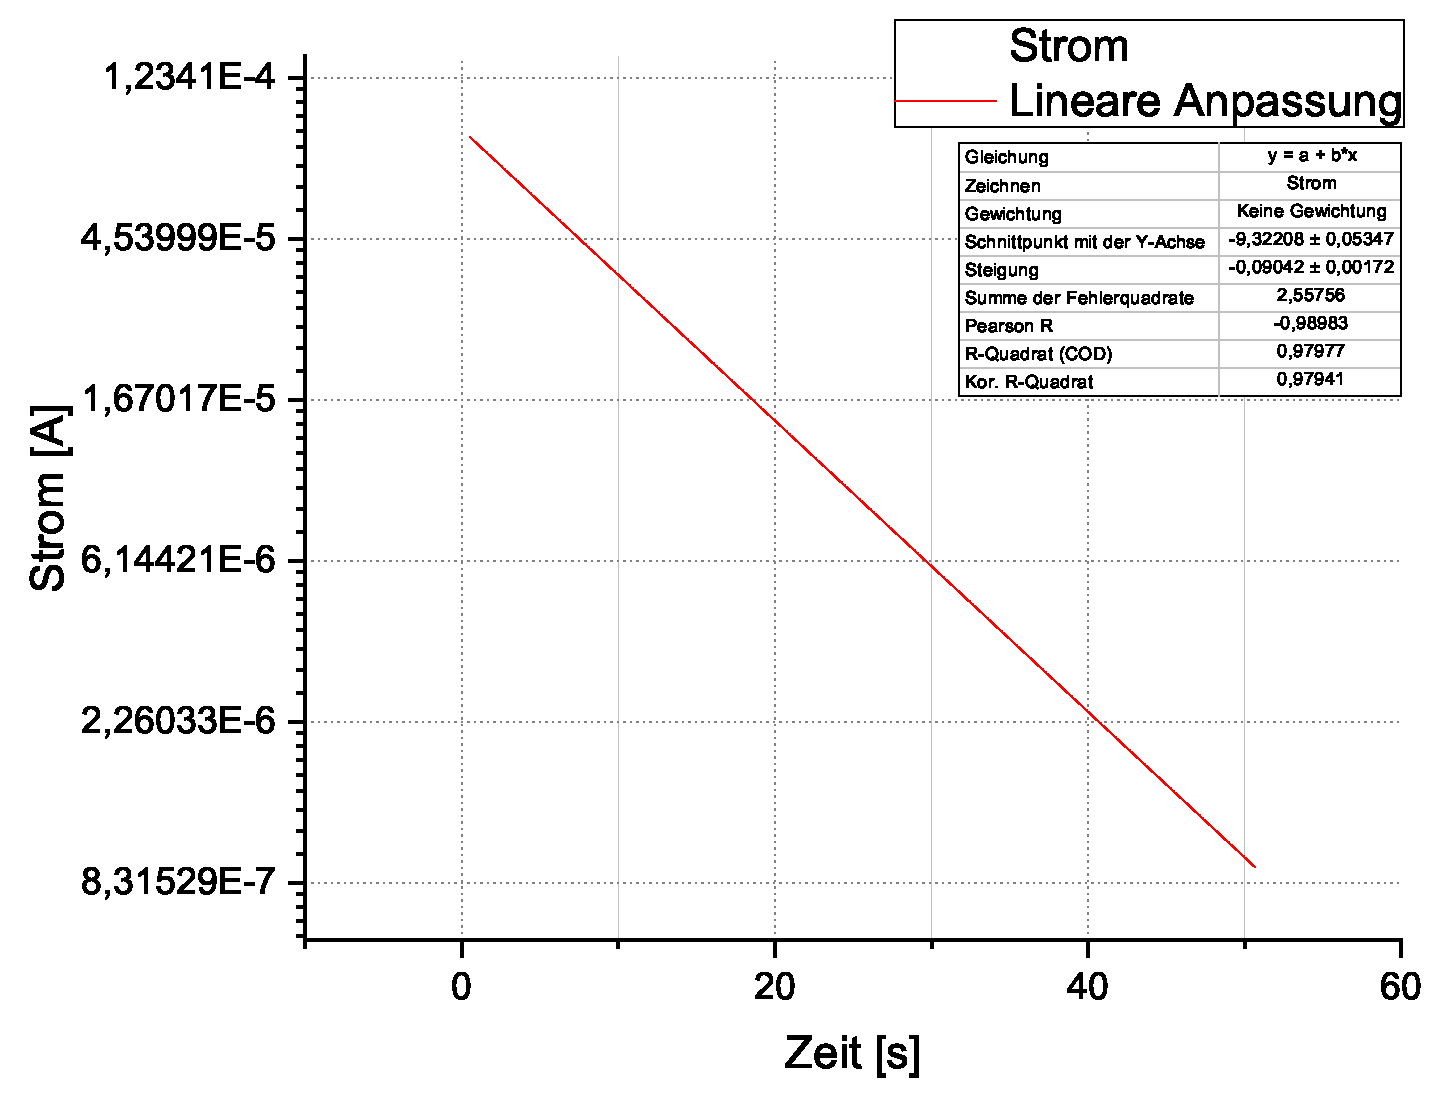
\includegraphics[scale=0.5]{Graph_Strom}
\caption{Halblogarithmische Darstellung des Stromes von Kondensator $C_2$ mit linearer Regression.}
\end{figure}

\begin{figure}[H]
\centering
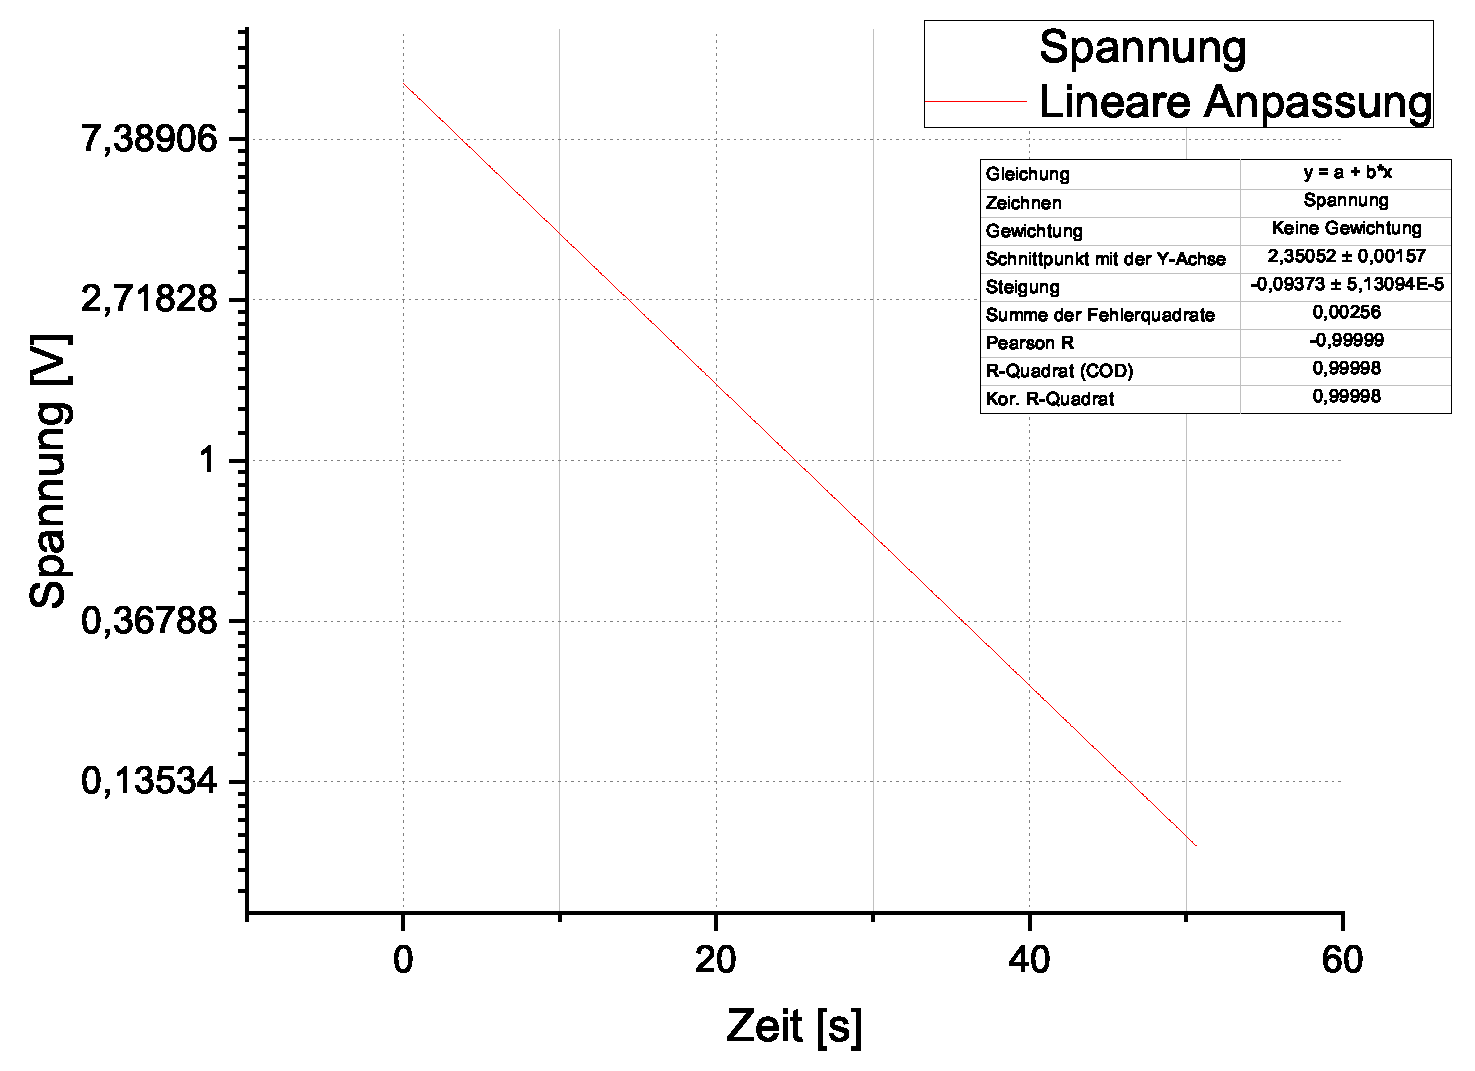
\includegraphics[scale=0.5]{Graph_Spannung}
\caption{Halblogarithmische Darstellung der Spannung von Kondensator $C_2$ mit linearer Regression.}
\end{figure}

Wir können nun mit der Steigung der Regressionsgeraden die Kapazität bestimmen. Dafür betrachten wir zunächst due Formeln für das Auf- (\ref{eq:auf}) und Entladen (\ref{eq:ent}) des Kondensators:

\begin{align}
U_C(t) &= U_0 \left(1 - e^{- \frac{1}{RC} \cdot t} \right) & I_C(t) &= \frac{U_0}{R} e^{\frac{1}{RC} \cdot t} \label{eq:auf} \\
U_C(t) &= U_0 e^{- \frac{1}{RC} \cdot t} & I_C(t) &= - \frac{U_0}{R} e^{\frac{1}{RC} \cdot t} \label{eq:ent}
\end{align}

Hierbei ist schnell zu erkennen, dass $b = - \frac{1}{RC}$ gilt, wodurch sich die Kapazität in beiden (allen) Fällen aus der Steigung wie fogt berechnet:

\begin{equation*}
b = - \frac{1}{RC} \Rightarrow C = - \frac{1}{R \cdot b}
\end{equation*}

Es ergibt sich dann:

Aus den Regressionen entnehmen wir $b_{Strom} = -0.09042 \pm 0.00172$ und $b_{Spannung} = -0.09373 \pm 5.13095 \cdot 10^{-5}$.

\begin{align*}
C_{Strom} &= \frac{1}{R \cdot b_{Strom}} = \frac{1}{104000 \Omega \cdot (-0.09042)} \approx 1.06341347217 \cdot 10^{-4} F \approx 106.3 \mu F \\
C_{Spannung} &= \frac{1}{R \cdot b_{Spannung}} = \frac{1}{104000 \Omega \cdot (-0.09373)} \approx 1.025859876 \cdot 10^{-4} F \approx 102.6 \mu F
\end{align*}

\end{flushleft}

\end{document}
